\documentclass{article}

\usepackage{graphicx}
\usepackage{hyperref}
\usepackage[margin=1.0in]{geometry}
\usepackage{float}

\title{\Huge Weighing a Whale}
\date{}

\begin{document}
\maketitle

\section{Finding the weight and density of a whale}

\begin{figure}
  Assume the length of the whale in the picture is 14 m long and the length has been measured accurately using drones.
  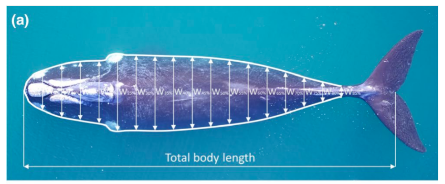
\includegraphics{whale_with_distances.png}
\end{figure}

\href{https://www.bbc.com/news/science-environment-49893849}{https://www.bbc.com/news/science-environment-49893849}
\\\\

1. Add this image to geogebra or desmos and adjust the scale appropriately. Have the horizontal axis of symmetry lie along the x-axis.

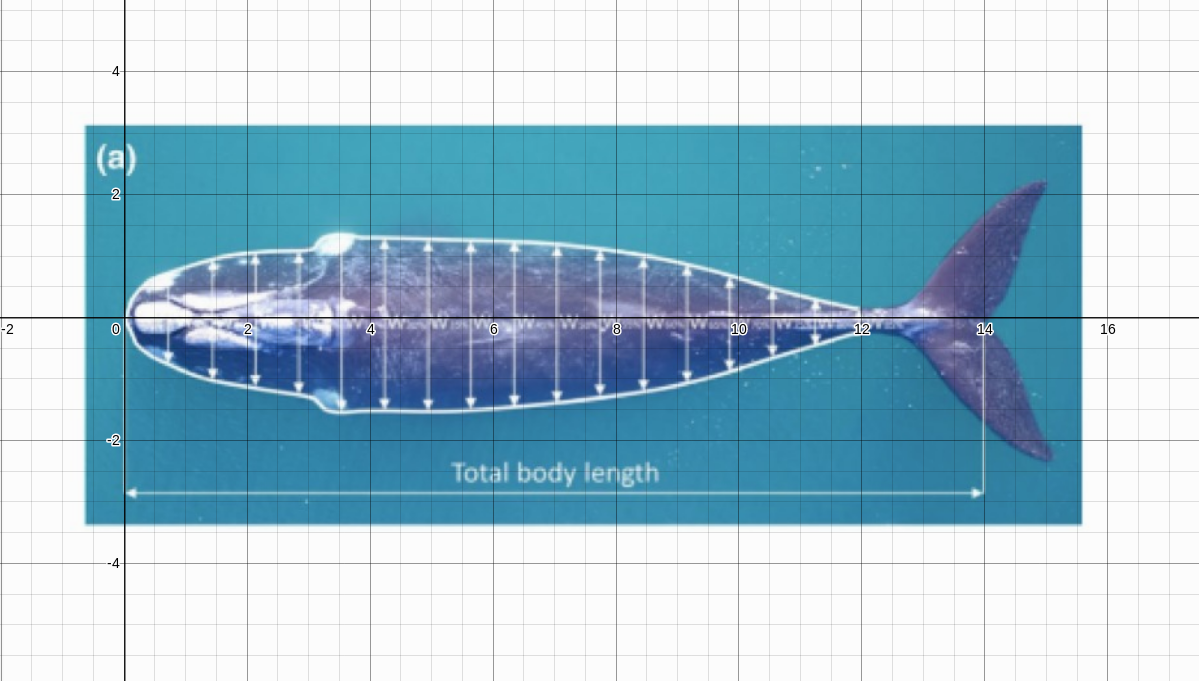
\includegraphics[scale=0.3]{desmos-whale.png}

The \textbf{girth} of a whale 

\end{document}
